\subsection{Firmware}

AVR is among the many architectures supported by the \texttt{gcc} compiler,
which makes it possible to write microcontroller software in C. The compiled
binary may be flashed to the chip using \texttt{avrdude}, a generic
on-chip memory uploader for AVR, paired with a hardware programmer such as
USBasp.

Conceptually, the firmware may be divided into several sections which interact
with each other at various stages of the program execution. These are:
\begin{itemize}
    \item The entry point, which configures the device and runs the main loop
    \item USART communication, which implements wrappers around the serial
    communication interface exposed by the microcontroller
    \item Command processing, which parses, validates and executes commands
    \item Motion handling, which contains code for calculating curves and
    controlling motors
    \item Feedback, which sends data to the controlling computer
\end{itemize}
All sections access a global object referred to as the \textit{machine state}.
It represents the current configuration of the CNC machine as a result of the
commands it received. It also contains the global error code, which is used to
implement a system of exceptions.

\begin{figure}[ht]
    \begin{center}
        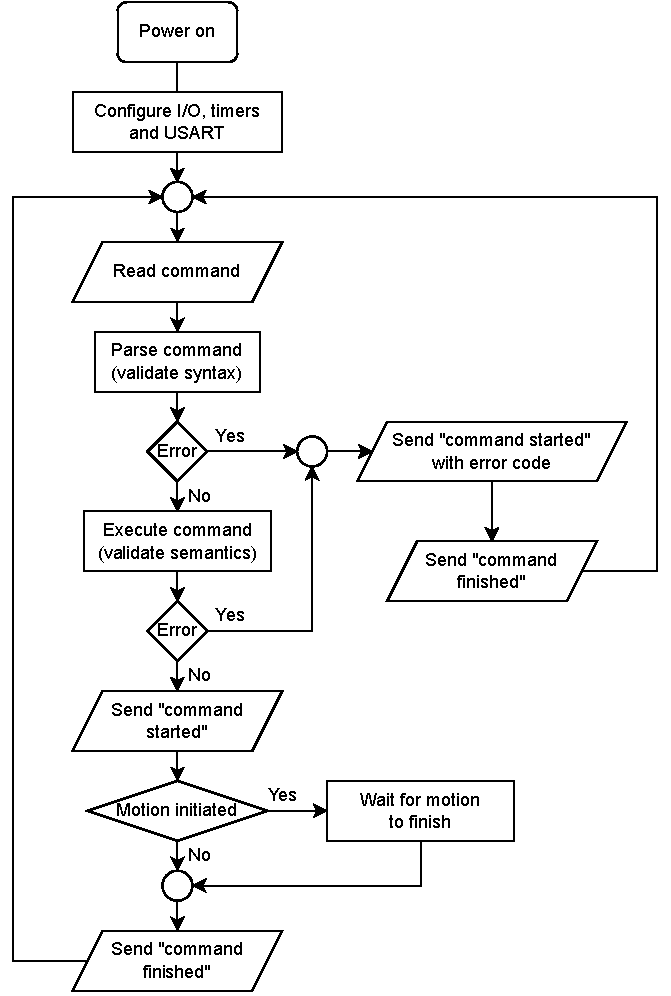
\includegraphics[width=0.47\linewidth]{firmware}
        \caption{A flowchart of the firmware's main loop.}
    \end{center}
\end{figure}

\subsubsection{Main loop}

A key feature of the firmware is its asynchronous nature. It must simultaneously
handle serial communication, command parsing, curve calculations, and periodic
feedback. As such, the majority of the program logic is implemented by means of
interrupts, which only last for a few milliseconds before returning. All
time-sensitive operations are guaranteed to run shortly after they are invoked.

With the above in mind, the main loop serves several purposes:
\begin{enumerate}
    \item It runs time-insensitive tasks which must be executed in between
    commands (command parsing and feedback)
    \item It burns CPU cycles when no interrupts are executing
    \item It clears the global error code once feedback is sent
\end{enumerate}

On power-up, before the main loop is entered, configuration code is executed.
This includes setting I/O pin directions, configuring timers and USART, and
enabling interrupts.

\subsubsection{USART communication}

\begin{figure}[ht]
    \begin{center}
        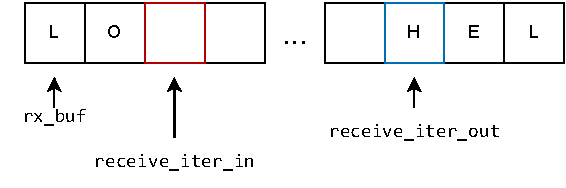
\includegraphics[width=0.6\linewidth]{usart}
        \caption{The USART circular buffer.}
    \end{center}
\end{figure}

To be able to process commands independently of when they are received, all
incoming data is placed in a buffer. It is a circular buffer which operates as a
FIFO queue. Incoming bytes are placed in the \texttt{receive\_iter\_in}
iterator, and the iterator is incremented. At a later time, they may be
retrieved in insertion order by reading from \texttt{receive\_iter\_out} and
incrementing it. If both iterators point to the same address, the buffer is
empty.

Commands are received by repeatedly reading from the receive buffer until a
newline character is encountered. If the buffer is empty, execution is stalled
until new data arrives. Collected characters are placed in a non-circular buffer
and terminated with a null byte.

Data transmission is done by calling a subroutine which takes a pointer to a
transmit buffer and the number of bytes to transmit. These are saved to a
statically allocated variable. Whenever the microcontroller is ready to send
the next byte, the pointer is dereferenced and incremented, and the length
counter is decremented. Transmission ends when the counter reaches zero.

To send feedback, the program statically allocates structures whose members
carry the feedback data. These structures are populated with data from the
program's global state and passed to the USART transmit subroutine, which sends
their binary representation to the control software.

\subsubsection{Command processing}

The command processor is a combined lexer-parser that populates a structure used
to describe a command. The production of a G-code command, in extended
Backus-Naur form, is as follows \cite{gcode}:
\footnotesize
\begin{verbatim}command ::= [block-delete], [line-number], {word | parameter-setting | comment};
word ::= letter, number;\end{verbatim}
\normalsize
(Remaining productions skipped for brevity.)

The parser attempts to parse each sub-production until the end of the buffer is
reached. It simultaneously checks for syntax errors and semantic errors. These
include:
\begin{itemize}
    \item Malformed input (failure to parse the root production)
    \item Unsupported syntax (parameter settings are not supported)
    \item Unsupported word letters (only letters from the set \texttt{G FIJXYZ}
    are supported)
    \item Unsupported G-word numbers (only a subset of G-code is implemented)
    \item Conflicting modal words (can't use rapid and arc movement at the same
    time)
    \item Duplicate non-modal words (can't have two X words)
\end{itemize}
The result of a successful parse is a structure describing which words were
present in the input and specifying their value. If there were no errors, this
structure is then passed to a subroutine responsible for command execution.

Execution is performed in a standardized order, guaranteeing consistent behavior
across machines. First, the machine state is updated to match the command. This
means setting the motion mode and other modes. Then, if the presence of the
words X, Y, or Z is detected, motion is initiated.

It is at this point that control is returned to the main loop, which generates
a feedback message about the command and waits for the motion to finish. The
loop then reiterates and another command is processed.

\subsubsection{Rapid and linear motion}

For each kind of motion implemented in the program, there are two subroutines:
the initializing subroutine and the handling subroutine. The former performs
initial calculations necessary to make the move and configures the device as
needed. The latter calculates the next step to be taken by the motors and runs
repeatedly at a frequency of several kilohertz. Motion ends when the handling
subroutine detects that it has reached its destination and resets the global
motion handler pointer to null.

\begin{figure}[ht]
    \centering
    \begin{minipage}{0.5\textwidth}
        \centering
        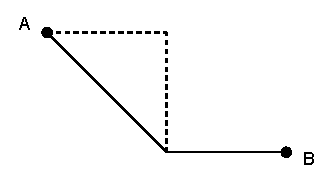
\includegraphics[width=0.76\textwidth]{rapid}
        \caption{Rapid motion.}
        \label{rapid}
    \end{minipage}\hfill
    \begin{minipage}{0.5\textwidth}
        \centering
        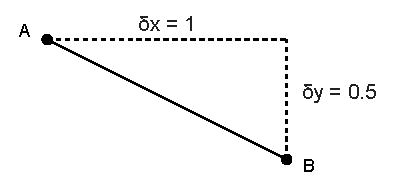
\includegraphics[width=0.9\textwidth]{linear}
        \caption{Linear motion.}
        \label{linear}
    \end{minipage}
\end{figure}

Rapid motion starts by configuring the direction of each of the motors. It then
moves the motor for each axis on every step until its respective destination
is reached. This allows it to move at $\sqrt{2}$ times the maximum speed of
a single motor when moving diagonally (see figure~\ref{rapid}).

Linear motion aims to limit the rate of movement for two of the three axes, so
that the destination point is reached by all axes at the same time. It does so
by calculating a fractional delta for each axis as such:
\begin{align*}
    \delta_{x} = \frac{\Delta_{x}}{max(\Delta_{x}, \Delta_{y}, \Delta_{z})} &&
    \delta_{y} = \frac{\Delta_{y}}{max(\Delta_{x}, \Delta_{y}, \Delta_{z})} &&
    \delta_{z} = \frac{\Delta_{z}}{max(\Delta_{x}, \Delta_{y}, \Delta_{z})}
\end{align*}
where $\Delta_n$ refers to the offset between the origin and the destination for
each axis.

On each step, the fractional delta is added to an accumulator which stores the
current position as a fixed-point non-integer number. Whenever the integer value
of the accumulator changes, its corresponding motor is made to move. As a
result, a straight line is plotted from the origin to the destination
(figure~\ref{linear}).

\subsubsection{Arc motion}

In G-code, arcs are described by specifying the arc center, the destination
point, and an implicit origin point. Not all combinations are valid; the origin
and the destination must be at a similar enough distance from the center,
otherwise an error is raised.

When the motion is initialized, the square of the distance between the center
and the destination becomes the \textit{reference radius}. The drawing algorithm
attempts to minimize the difference between the current measured radius and the
reference radius, while at the same time moving forward. This causes it to move
in a circular path.

On each step, the current direction of travel is calculated. For clockwise arcs,
this is:
\begin{gather*}
    \delta_x = \begin{cases}
        1 & \text{if } (x \geq 0 \land y < 0) \lor (x < 0 \land y \leq 0)\\
        -1 & \text{otherwise}
    \end{cases}
    \\
    \delta_y = \begin{cases}
        1 & \text{if } (x \geq 0 \land y < 0) \lor (x > 0 \land y \geq 0)\\
        -1 & \text{otherwise}
    \end{cases}
\end{gather*}
where $x$ and $y$ are coordinates relative to the arc center. Once this is done,
there are three possible moves to be considered. The algorithm choses the one
whose radius is the closest to the reference radius (see figure~\ref{arc}).
\begin{align*}
    R^2_x &= (x + \delta_x)^2 + y^2 \\
    R^2_{xy} &= (x + \delta_x)^2 + (y + \delta_y)^2 \\
    R^2_y &= x^2 + (y + \delta_y)^2
\end{align*}

\begin{figure}[ht]
    \begin{center}
        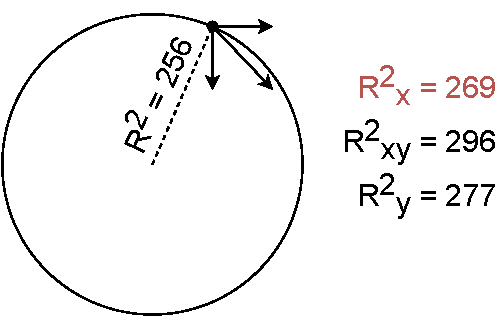
\includegraphics[width=0.5\linewidth]{arc}
        \caption{Possible steps when drawing an arc.}
        \label{arc}
    \end{center}
\end{figure}

The algorithm terminates once the destination point has been reached. This is
always possible because the reference radius is measured against the
destination, not the origin. Also note that this algorithm is able to recover
from a situation where the starting point is not strictly in the arc.
